%=================================================
\sectionDark{ID3}
%=================================================
\begin{frame}
  \frametitle{TDIDT\footnote{Diapositiva sacada del temario de SGDI}}
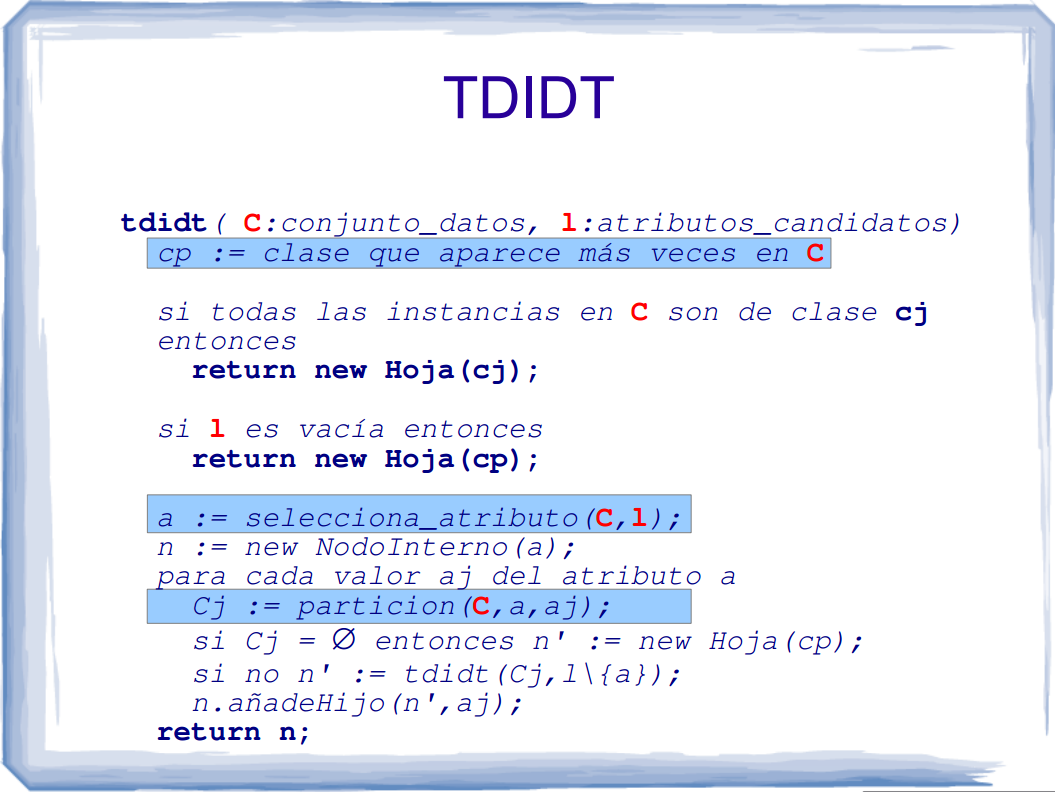
\includegraphics[width=\textwidth]{./images/c45/esquemaTDIDT.png}
\end{frame}

\begin{frame}
  \frametitle{ID3\footnote{Diapositiva sacada del temario de SGDI}}
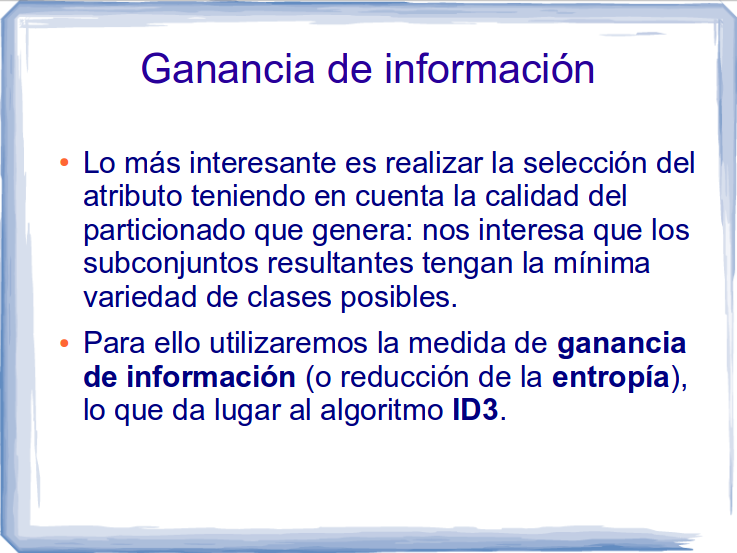
\includegraphics[width=\textwidth]{./images/c45/esquemaID3.png}
\end{frame}

%=================================================
\sectionDark{C4.5}
%=================================================
\begin{frame}
  \frametitle{C4.5}
  El algoritmo ID3 es mejorado por el C4.5. Esta mejora, aparte de la
  optimizaci�n de partes de c�digo, incluye\footnote{Art�culo con las bases del algoritmo \cite{quinlan1986induction}}:
  \begin{itemize}
  \item Permitir atributos continuos.
  \item Permitir dar un peso diferente a cada atributo.
  \item Permitir a una instancia no tener definido un valor en sus
    atributos.
  \item Mejorar la selecci�n del atributo clasificador.
  \item Realizar una poda del �rbol despu�s de la creaci�n.
  \end{itemize}
\end{frame}

\begin{frame}[fragile]
  \frametitle{Algoritmo C4.5\footnote{Obtenido del libro \cite{quinlan2014c4} y su review \cite{salzberg1994c4}}}
  \begin{tikzpicture}
    \tikzpicdimlarge
    \only<1->{\node[] (def) at (0.5,6) {
        \begin{minipage}{0.9\textwidth}
          \textcolor{purple}{\textbf{Split y Funciones Test:}}
          Para dividir en subconjuntos las instancias test se divide el
          dominio donde haya mayor ganancia de informaci�n. Esta
          divisi�n se traduce en funciones test de tipo $x > 40$ � $x
          < 4$, y para atributos discretos $ x = soleado$. 
        \end{minipage}
      };}

    \only<2->{\node[] (def) at (0.5,2) {
        \begin{minipage}{0.9\textwidth}
          \textcolor{purple}{\textbf{Selecci�n del atributo:}}
          La selecci�n del atributo por el que dividir consiste en
          escoger el atributo con mayor ganancia de informaci�n
          normalizado y ponderado. \\

          Para ello, se tiene en cuenta la proporci�n de instancias
          que queda en cada rama para el atributo candidato y el peso
          de importancia dado a dicho atributo.
          Siendo $D$ el conjunto de instancias, la f�rmula para el
          atributo $i$ queda:
          $$ Ganancia_i = Peso_i * \sum_j \frac{|D_j|}{|D|} * Info_j $$
        \end{minipage}
      };}

  \end{tikzpicture}
\end{frame}

\begin{frame}[fragile]
  \frametitle{Ejemplo --  ID3 vs C4.5 (atributos continuos)}
\begin{tikzpicture}
\tikzpicdimlarge
\only<1->{\node[] () at (0,9)
  {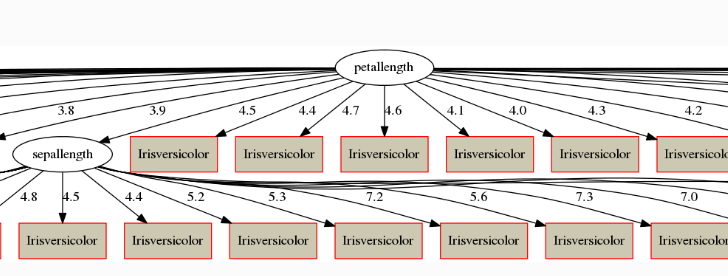
\includegraphics[width=0.65\textwidth]{./images/c45/ID3iris.png}};}
\only<2->{\node[] () at (0,5)
  {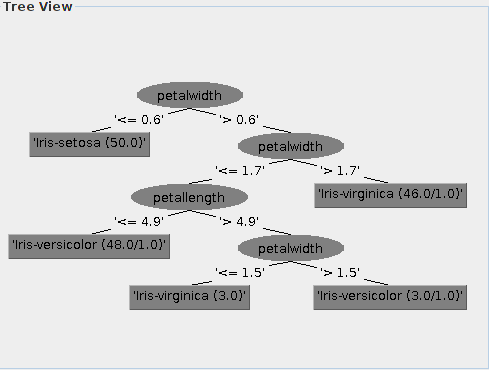
\includegraphics[width=0.65\textwidth]{./images/c45/C45tree.png}};}

\end{tikzpicture}
\end{frame}

\begin{frame}
  \frametitle{C4.8 (J48): Mejoras a C4.5}
  \begin{tikzpicture}
    \tikzpicdimlarge
    \only<1->{\node[] (def) at (0.5,6) {
        \begin{minipage}{0.9\textwidth}
          \textcolor{purple}{\textbf{Problemas:}}\\
        ``The accuracy of T2's trees rivalled or surpassed C4.5's on 8
        of the 15 datasets, including all but one of the datasets
        having only continuous attributes.'' \cite{auer1995theory}\\

        ``C4.5's performance was significantly improved on two data
        sets [...] using the entropy discretization method and did no
        significantly degrade on any datasets [...] We conjeture that
        the C4.5 induction algorithm is not taking full advantage of
        possible local discretization.'' \cite{dougherty1995supervised}
        \end{minipage}
      };}
    \only<2->{\node[] (def) at (0.5,1.8) {
        \begin{minipage}{0.9\textwidth}
          \textcolor{purple}{\textbf{Soluci�n \cite{quinlan1996improved}:}}
          \begin{itemize}
            \item Aumentar el coste de usar atributos continuos
              disminuyendo el peso de importancia del atributo.
            \item Simplificar la divisi�n de un atributo continuo, en
              lugar de maximizar la ganacia, basta con superar un
              l�mite.
            \item Se a�ade el generador de reglas.
          \end{itemize}
        \end{minipage}
      };}
\end{tikzpicture}
\end{frame}

%=================================================
\sectionDark{C5.0}
%=================================================

\begin{frame}
  \frametitle{C5.0}
% Mejoras
  C5.0 tiene licencia comercial y licencia GPL para un solo proceso.\\
   \textcolor{purple}{\textbf{Mejoras \footnote{Basado en
         \cite{pandya2015c5} y la p�gina oficial del autor \cite{quinlanURL}
         http://www.rulequest.com/ }:}}
\begin{itemize}
\item Aumenta el rendimiento del algoritmo.
\item Reduce el consumo de memoria local y total.
\item Devuelve �rboles de clasificaci�n reducidos.
\item Poda atributos irrelevantes para la clasificaci�n.
\item Hace la ponderaci�n de atributos m�s precisa.
\item Agrupa valores de atributos discretos en una misma rama.
\item Genera reglas con m�s acierto que las de C4.8.
\item Facilita la aplicaci�n de t�cnicas como bagging y boosting,
  mejorando sus resultados.\footnote{\cite{freund1999alternating}}
\end{itemize}
\end{frame}

\begin{frame}[fragile,fragile,fragile]
\frametitle{C5.0: Ejemplo en R}
\begin{tikzpicture}
\tikzpicdimlarge

\only<1->{\node[] (def) at (0.5,9) {
\begin{minipage}{0.8\textwidth}
crx$<$-read.table(file="./crx.data",header=FALSE,sep=",") \\
head( crx, 6 ) \\
\end{minipage}
};}
\only<2->{\node[] (def) at (0.5,7.8) {
\begin{minipage}{0.8\textwidth}
crx $<$- crx[ sample( nrow( crx ) ), ] \\
X $<$- crx[,1:15] \\
y $<$- crx[,16] \\
\end{minipage}
};}
\only<3->{\node[] (def) at (0.5,6) {
\begin{minipage}{0.8\textwidth}
trainX $<$- X[1:600,] \\
trainy $<$- y[1:600] \\
testX $<$- X[601:690,] \\
testy $<$- y[601:690] \\
\end{minipage}
};}
\only<4->{\node[] (def) at (0.5,4.5) {
\begin{minipage}{0.8\textwidth}
\textbf{library(C50) \\
model $<$- C50::C5.0( trainX, trainy ) \\
summary( model )}
\end{minipage}
};}
\only<1->{\node[] (def) at (0.5,2) {
\begin{minipage}{\textwidth}
Ejemplo de C5.0 en R obtenido de:
\myurl{http://connor-johnson.com}
\end{minipage}
};}


\end{tikzpicture}
\end{frame}




